\section{Sprint 6}
\subsection{Sprint start}


\subsection{Sprint burndown}



\begin{figure}[H]
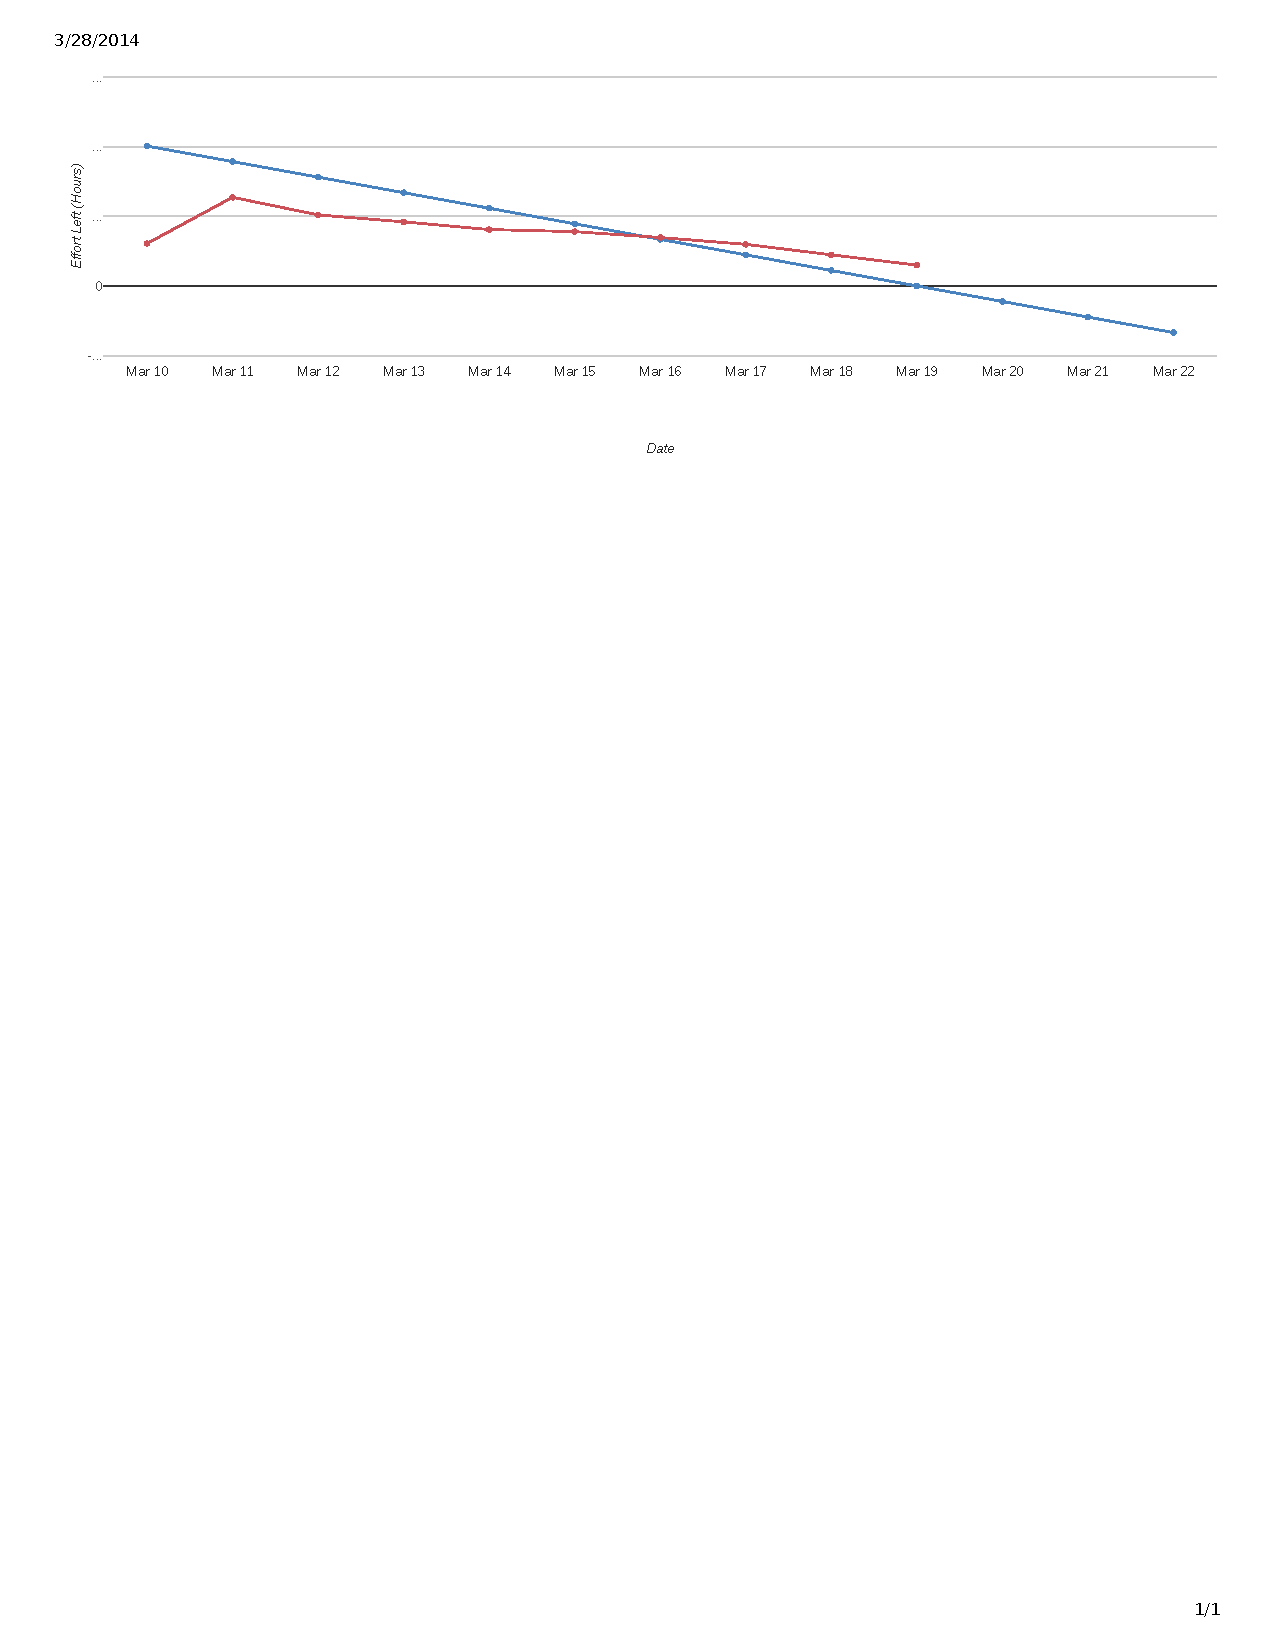
\includegraphics[width=\textwidth, trim= 1cm 21cm 1cm 1cm, clip=true]{ch/projectManagement/fig/burndown4.pdf}
\caption{Sprint 6 burndown chart}
\label{fig:sprint6burndown}
\end{figure}

\subsection{Sprint backlog}

The backlog and time usage result.

\begin{table}[H]
	\begin{tabular}{|l|p{7cm}|p{2.2cm}|p{1.5cm}|p{1.5cm}|}%
		\hline \bfseries User story & \bfseries Details & \bfseries Hours\newline estimated & \bfseries Hours spent & \bfseries Hours left
		\csvreader[head to column names]{ch/projectManagement/sec/sprints/sprint6/userstories.csv}{}% use head of csv as column names
		{\\\hline \id & \title & \estimated & \spent & \left} \\\hline% specify your coloumns here
	\end{tabular}
    \caption{Sprint 3 backlog}
\end{table}


\subsection{Sprint end}